%!TEX root = stokes_paper.tex

\section{Examples \label{sec:results}}
In this section, we test the lightning Stokes solver on various sample problems found in the literature. For each example, we present contour plots for the stream function $\psi$ superimposed on a color plot of the velocity magnitude $\sqrt{u^2+v^2}$. We use black contours for the first Moffatt eddy, and subsequent ones are highlighted in yellow. We show a portion of the nearest poles indicated by red dots. The plots of the linear least-squares (weighted) residual indicate root-exponential convergence as expected. We also provide a close-up of the eddies.

Inverting the sign of the boundary data $(h,k)=(\psi_0(z_i), U_t(z_i))$ and $\vec{g}=(U(z_i), -V(z_i))$ would have the effect of reversing the direction of the flow, since \eqref{eq:bih}--\eqref{eq:bcs} is linear. Therefore, the streamline pattern and the velocity magnitude plot would appear unaltered if these flipped conditions were imposed instead.   

\subsection{Lid-driven square cavity}
In Figure \ref{fig:ldc} we show a lid-driven cavity, where the fluid is enclosed between unmovable walls but one of them moves tangentially to the fluid as the stirring mechanism. Here, the domain is the square $\Omega=[-1,1]^2$, where we have a no-slip BC with $\psi=0$ on the bottom, left and right edges, and we impose $u=1$ and $\psi=0$ on the top edge. In this first example, the gradient data $k(x,y)$ is discontinuous, so $\psi$ presents point-singularities at $(\pm 1, 1)$. On the bottom corners, $(\pm 1,-1)$, there are (weaker) point-singularities caused by the formation of Moffatt eddies, on which our adaptive strategy has put less poles than the ones on the top.


\subsection{Lid driven triangular cavity}
The example from Figure \ref{fig:wedge} is quite similar to the previous one in terms of boundary conditions and singularities, except that the bottom surface has been collapsed to a single point. Here, the domain is the wedge $\Omega = \{z= i r e^{i\theta}: r<1, -\alpha \leq \theta\leq \alpha\}$ with total angle $2\alpha = 28.5^\circ$. This particular setup was chosen for comparison with experimental images from \cite{taneda79} for a flow with $\text{Re}=1.7\times10^{-1}$ where the stirring mechanism was a rotating cylinder placed at the top surface.

In Figure \ref{fig:step} we have the L-shaped domain $\Omega = [-1,0] \times [0,1] \cup [0,5]\times[-1,1]$ that resembles a pipe with a sudden expansion or a step. Fully-developed parabolic profiles are imposed on the inflow and outflow such that mass is conserved, i.e. $(u,v)=(1-(2y-1)^2,0)$ at $x=-1$, $(u,v)=((1-y^2)/2,0)$ at $x=5$, and for the remaining surfaces we impose a no-slip BC with $\psi_0=2/3$ at $y=1$ and $\psi_0=0$ on the other surfaces. We observe more poles clustered near the re-entrant corner $(0,0)$, where the pressure becomes unbounded, and the formation of Moffatt eddies at $(0,-1)$. In order to make this example work, it was crucial to introduce a fake corner at $(0,1)$.


\begin{figure}[H]
	
	\centering
	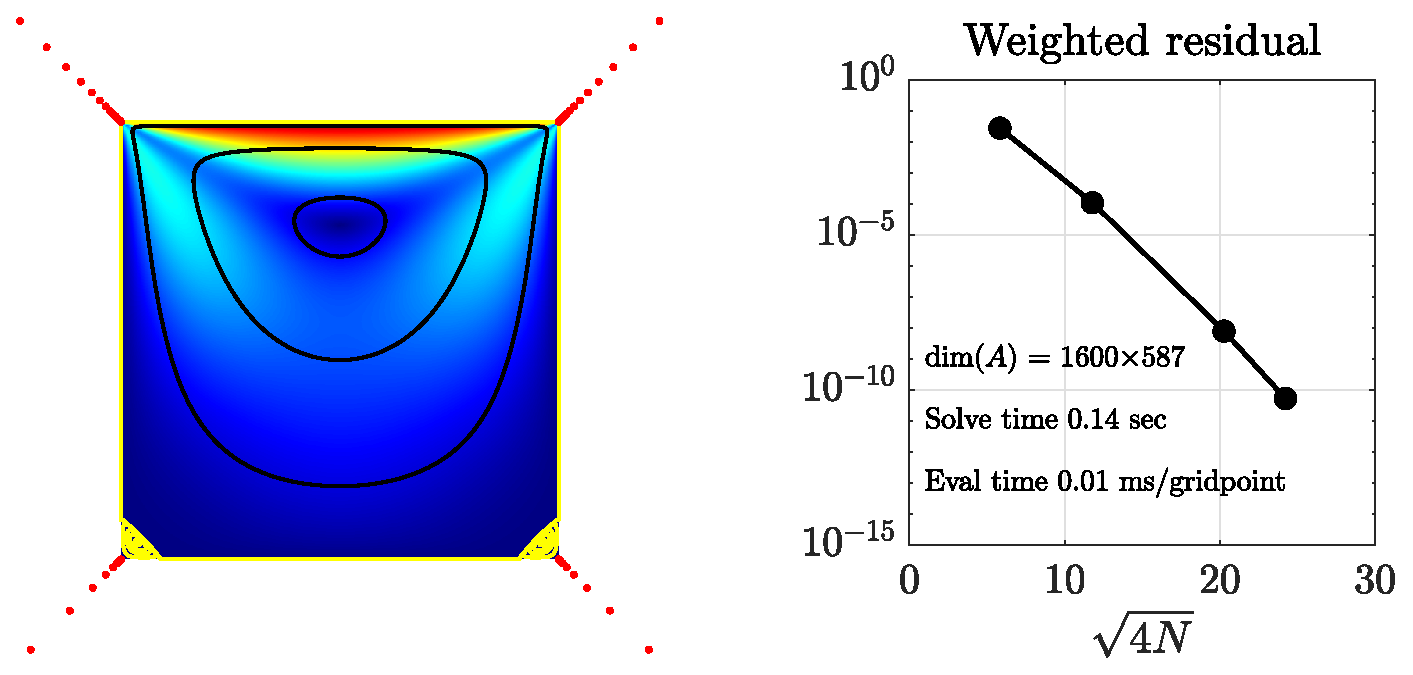
\includegraphics[width=\linewidth]{Figures/ldc}
	
	\vspace{2em}
	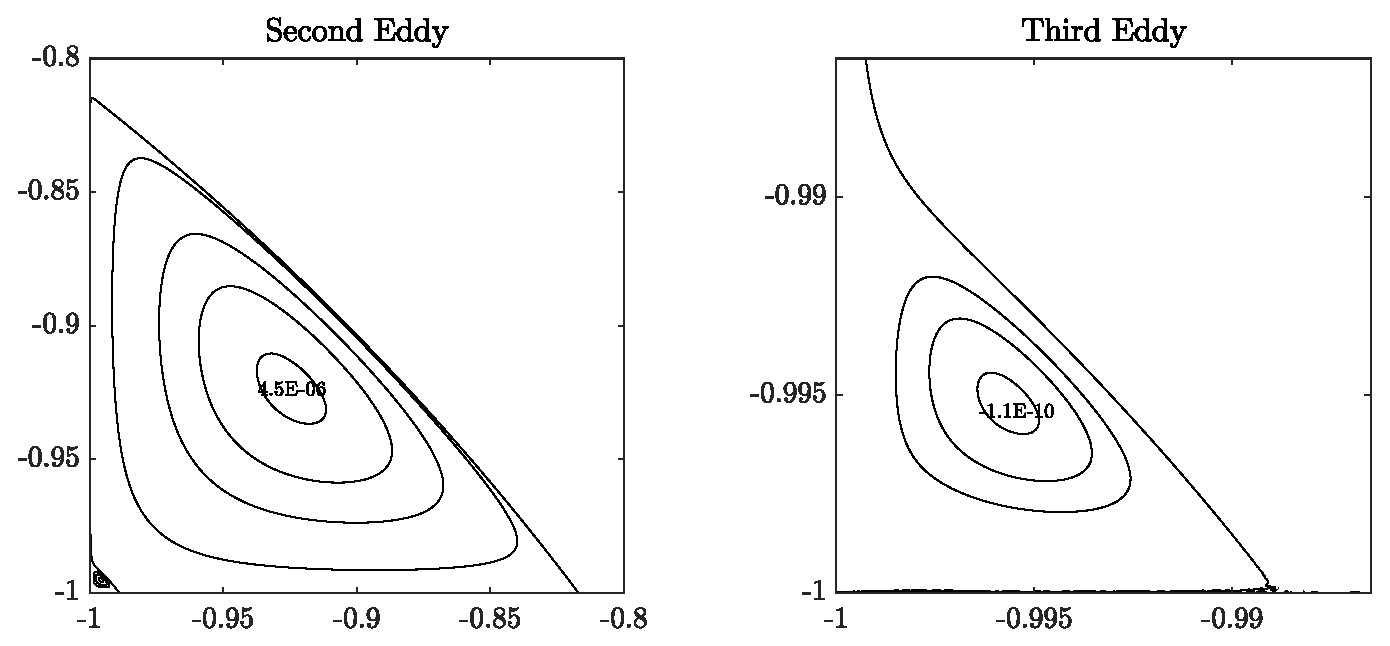
\includegraphics[width=\linewidth]{Figures/ldc_eddy}
	
	%\caption{Stokes flow inside a square lid-driven cavity. In this example, a fluid is enclosed inside a cavity, whose top lid moves from left to right with unit speed, and no-slip boundary conditions are imposed on the other three edges. The corner singularities induced by the discontinuity in the derivatives of $\psi$, together with the simplicity of the domain, make this problem an ideal test	case.}
	\caption{.}
	\label{fig:ldc}
\end{figure} 

\begin{figure}[H]
	\centering
	\includegraphics[width=\linewidth]{Figures/ldc_loglog}
%	\caption{Log-log plot along the $45^\circ$ line, where $r$ is distance measured from the point $(-1,-1)$. At $r=2\sqrt{2}$ we have imposed $\psi=0$}
	\caption{.}
	\label{fig:ldc_loglog}
\end{figure}

\begin{figure}[H]
	
	\centering
	\begin{minipage}{0.45\linewidth}
		\centering
		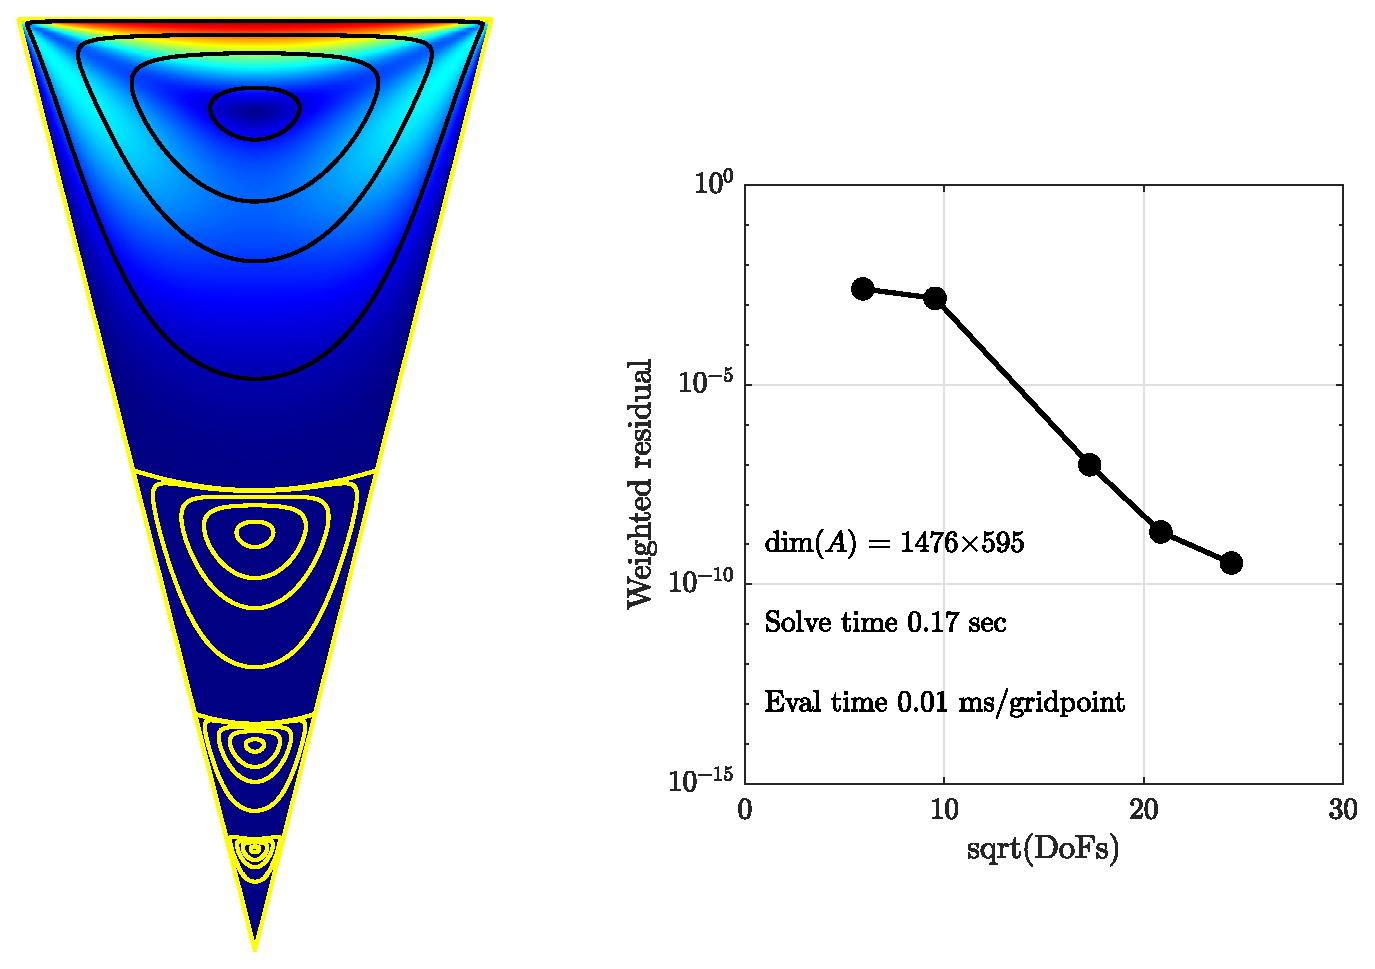
\includegraphics[width=\linewidth]{Figures/wedge}
	\end{minipage}
	\hfill
	\begin{minipage}{0.45\linewidth}
		\centering
		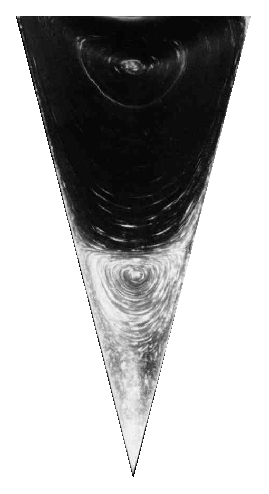
\includegraphics[width=0.6\linewidth]{Figures/wedge_exp}
	\end{minipage}

	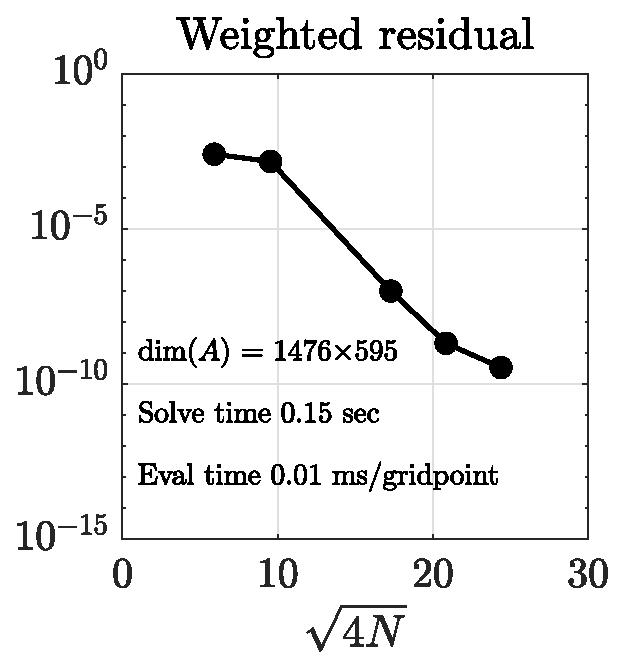
\includegraphics[width=0.5\linewidth]{Figures/wedge_conv}
	\caption{Stokes flow inside a wedge of total angle $28.5^\circ$. The top lid moves from left to right with unit speed and no-slip boundary conditions are imposed at the other 2 surfaces. For comparison, the first two eddies have been observed experimentally by Taneda in \cite[Fig.~19]{taneda79}, also included in \cite[Fig.~10]{vandyke82}, for a very similar setup driven by a rotating cylinder with $\text{Re}=1.7\times10^{-1}$.}
	\label{fig:wedge}
\end{figure} 

\begin{figure}[H]
	\centering
	\includegraphics[width=\linewidth]{Figures/wedge_loglog}
	%	\caption{Log-log plot along the $45^\circ$ line, where $r$ is distance measured from the point $(-1,-1)$. At $r=2\sqrt{2}$ we have imposed $\psi=0$}
	\caption{.}
	\label{fig:wedge_loglog}
\end{figure}

\begin{figure}[H]
	\centering
	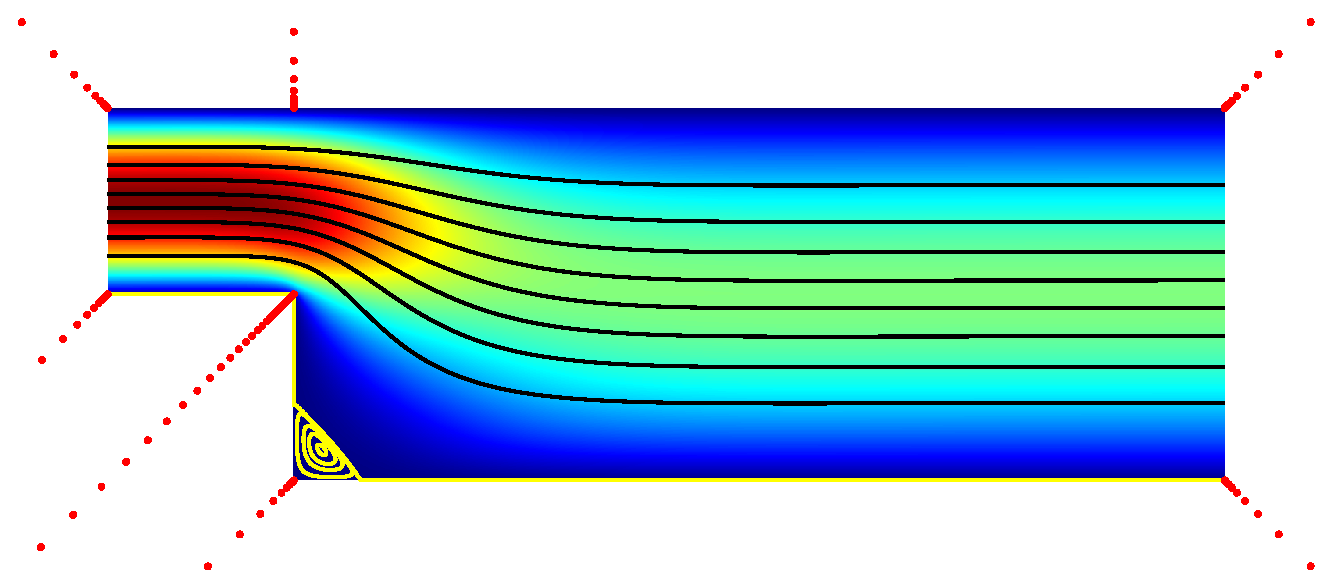
\includegraphics[width=\linewidth]{Figures/step}
	
	\vspace{2em}
	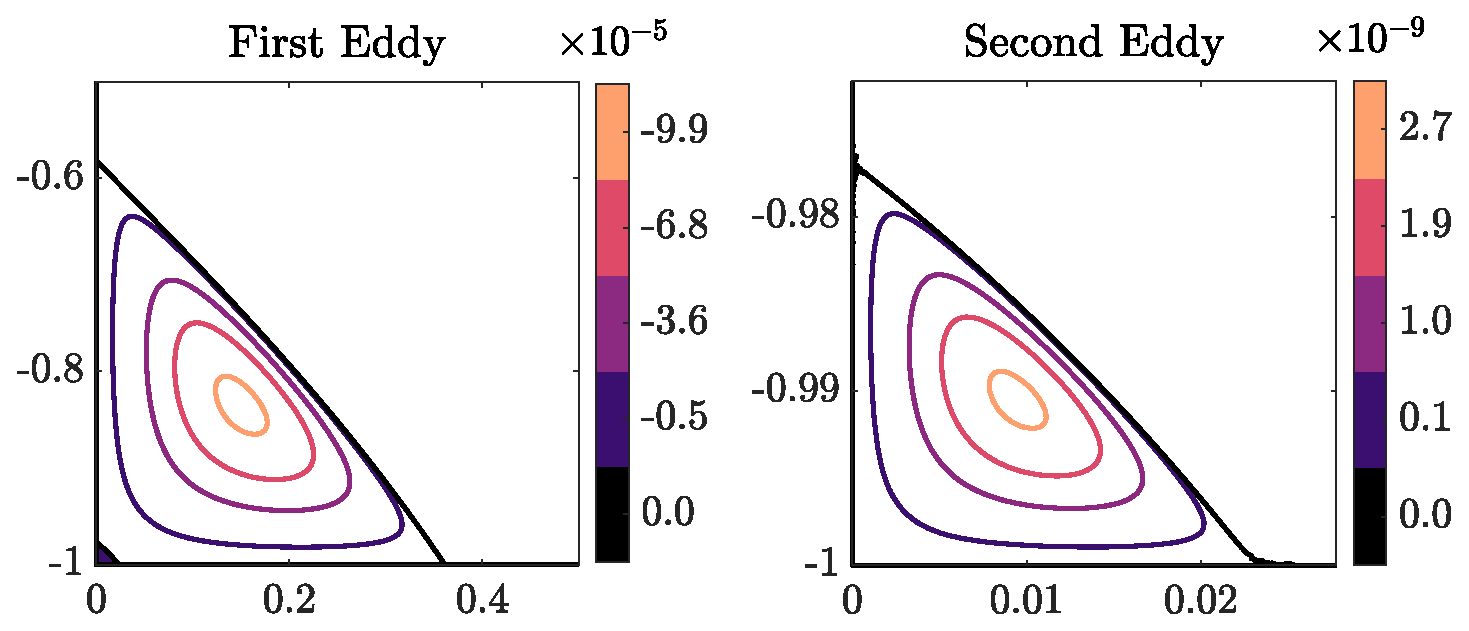
\includegraphics[width=\linewidth]{Figures/step_eddy}
	
	\vspace{2em}
	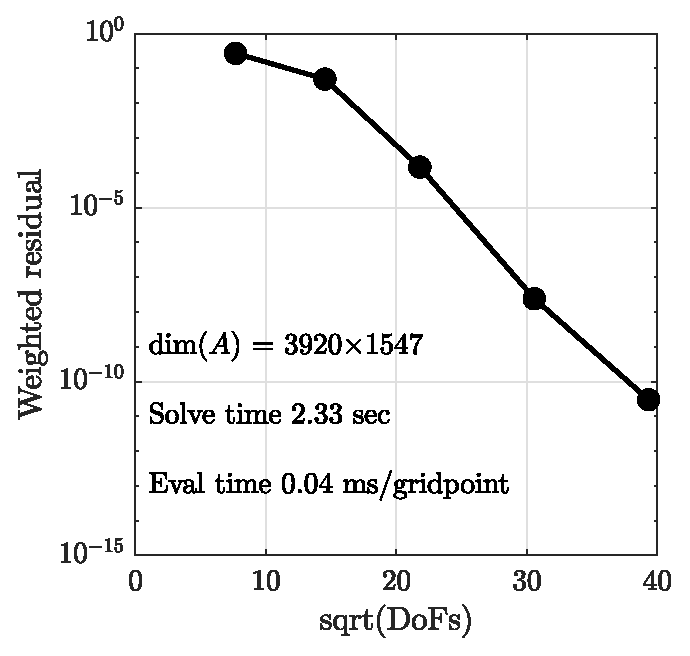
\includegraphics[width=0.5\linewidth]{Figures/step_conv}

	\caption{Stokes flow over a step. A parabolic profile is prescribed at the inflow and at the outflow, and a no-slip condition is imposed on the rest of the walls. At the re-entrant corner the pressure and the derivatives of the velocity become unbounded.}
	\label{fig:step}
\end{figure} 

\section{Unbounded domains \label{sec:unbounded}}


\begin{figure}[H]
	\centering
	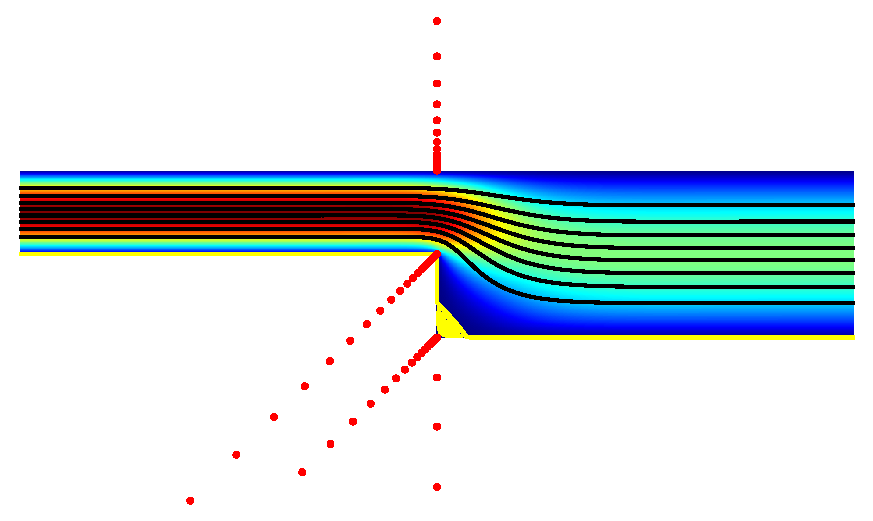
\includegraphics[width=\linewidth]{Figures/chan}
	
	\vspace{2em}
	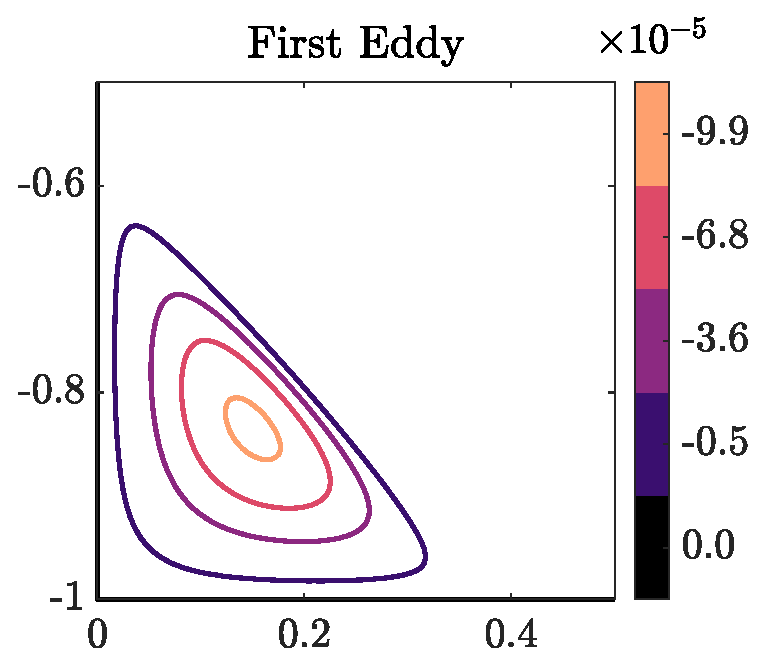
\includegraphics[width=0.45\linewidth]{Figures/chan_eddy}
	\hfill
	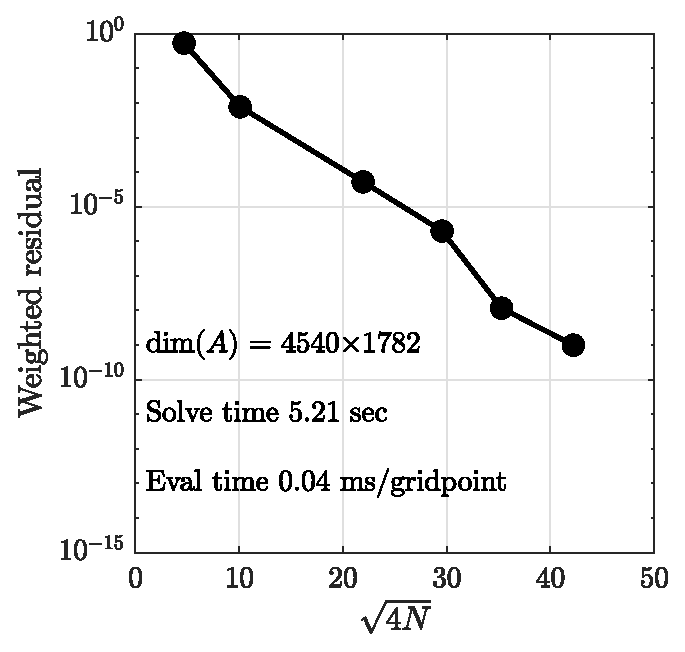
\includegraphics[width=0.45\linewidth]{Figures/chan_conv}

	\caption{Stokes flow inside an infinitely long pipe with an expansion.}
	\label{fig:chan}
\end{figure} 

\section{Multiply connected domains \label{sec:multiply}}


